\documentclass[review]{elsarticle}\usepackage[]{graphicx}\usepackage[]{color}
%% maxwidth is the original width if it is less than linewidth
%% otherwise use linewidth (to make sure the graphics do not exceed the margin)
\makeatletter
\def\maxwidth{ %
  \ifdim\Gin@nat@width>\linewidth
    \linewidth
  \else
    \Gin@nat@width
  \fi
}
\makeatother

\definecolor{fgcolor}{rgb}{0.345, 0.345, 0.345}
\newcommand{\hlnum}[1]{\textcolor[rgb]{0.686,0.059,0.569}{#1}}%
\newcommand{\hlstr}[1]{\textcolor[rgb]{0.192,0.494,0.8}{#1}}%
\newcommand{\hlcom}[1]{\textcolor[rgb]{0.678,0.584,0.686}{\textit{#1}}}%
\newcommand{\hlopt}[1]{\textcolor[rgb]{0,0,0}{#1}}%
\newcommand{\hlstd}[1]{\textcolor[rgb]{0.345,0.345,0.345}{#1}}%
\newcommand{\hlkwa}[1]{\textcolor[rgb]{0.161,0.373,0.58}{\textbf{#1}}}%
\newcommand{\hlkwb}[1]{\textcolor[rgb]{0.69,0.353,0.396}{#1}}%
\newcommand{\hlkwc}[1]{\textcolor[rgb]{0.333,0.667,0.333}{#1}}%
\newcommand{\hlkwd}[1]{\textcolor[rgb]{0.737,0.353,0.396}{\textbf{#1}}}%

\usepackage{framed}
\makeatletter
\newenvironment{kframe}{%
 \def\at@end@of@kframe{}%
 \ifinner\ifhmode%
  \def\at@end@of@kframe{\end{minipage}}%
  \begin{minipage}{\columnwidth}%
 \fi\fi%
 \def\FrameCommand##1{\hskip\@totalleftmargin \hskip-\fboxsep
 \colorbox{shadecolor}{##1}\hskip-\fboxsep
     % There is no \\@totalrightmargin, so:
     \hskip-\linewidth \hskip-\@totalleftmargin \hskip\columnwidth}%
 \MakeFramed {\advance\hsize-\width
   \@totalleftmargin\z@ \linewidth\hsize
   \@setminipage}}%
 {\par\unskip\endMakeFramed%
 \at@end@of@kframe}
\makeatother

\definecolor{shadecolor}{rgb}{.97, .97, .97}
\definecolor{messagecolor}{rgb}{0, 0, 0}
\definecolor{warningcolor}{rgb}{1, 0, 1}
\definecolor{errorcolor}{rgb}{1, 0, 0}
\newenvironment{knitrout}{}{} % an empty environment to be redefined in TeX

\usepackage{alltt}
%% Numbered
%\bibliographystyle{model1-num-names}

%% Numbered without titles
%\bibliographystyle{model1a-num-names}

%% Harvard
%\bibliographystyle{model2-names.bst}\biboptions{authoryear}

%% Vancouver numbered
%\usepackage{numcompress}\bibliographystyle{model3-num-names}

%% Vancouver name/year
%\usepackage{numcompress}\bibliographystyle{model4-names}\biboptions{authoryear}

%% APA style
%\bibliographystyle{model5-names}\biboptions{authoryear}

%% AMA style
%\usepackage{numcompress}\bibliographystyle{model6-num-names}

%% `Elsevier LaTeX' style
\bibliographystyle{elsarticle-num}
%%%%%%%%%%%%%%%%%%%%%%%
\usepackage{amsmath}
\usepackage[T1]{fontenc}
\usepackage{lmodern}
\usepackage{amssymb,amsmath}
\usepackage{ifxetex,ifluatex}
\usepackage{lscape}
\usepackage{fixltx2e} % provides \textsubscript
% use upquote if available, for straight quotes in verbatim environments
\IfFileExists{upquote.sty}{\usepackage{upquote}}{}
\ifnum 0\ifxetex 1\fi\ifluatex 1\fi=0 % if pdftex
  \usepackage[utf8]{inputenc}
\else % if luatex or xelatex
  \ifxetex
    \usepackage{mathspec}
    \usepackage{xltxtra,xunicode}
  \else
    \usepackage{fontspec}
  \fi
  \defaultfontfeatures{Mapping=tex-text,Scale=MatchLowercase}
  \newcommand{\euro}{€}
\fi
% use microtype if available
\IfFileExists{microtype.sty}{\usepackage{microtype}}{}
\usepackage[margin=1in]{geometry}
\usepackage{longtable,booktabs}
\usepackage{graphicx}
% Redefine \includegraphics so that, unless explicit options are
% given, the image width will not exceed the width of the page.
% Images get their normal width if they fit onto the page, but
% are scaled down if they would overflow the margins.
\makeatletter
\def\ScaleIfNeeded{%
  \ifdim\Gin@nat@width>\linewidth
    \linewidth
  \else
    \Gin@nat@width
  \fi
}
\makeatother
\let\Oldincludegraphics\includegraphics
{%
 \catcode`\@=11\relax%
 \gdef\includegraphics{\@ifnextchar[{\Oldincludegraphics}{\Oldincludegraphics[width=\ScaleIfNeeded]}}%
}%
\ifxetex
  \usepackage[setpagesize=false, % page size defined by xetex
              unicode=false, % unicode breaks when used with xetex
              xetex]{hyperref}
\else
  \usepackage[unicode=true]{hyperref}
\fi
\hypersetup{breaklinks=true,
            bookmarks=true,
            pdfauthor={},
            pdftitle={},
            colorlinks=true,
            citecolor=blue,
            urlcolor=blue,
            linkcolor=magenta,
            pdfborder={0 0 0}}
\urlstyle{same}  % don't use monospace font for urls
\setlength{\parindent}{0pt}
\setlength{\parskip}{6pt plus 2pt minus 1pt}
\setlength{\emergencystretch}{3em}  % prevent overfull lines
\setcounter{secnumdepth}{0}
\usepackage{pdfpages}
\usepackage{xcolor}      % use if color is used in text
\usepackage{endnotes}
\usepackage{graphicx}   % need for figures
\usepackage{verbatim}   % useful for program listings
\usepackage{hyperref}   % use for hypertext links, including those to external documents and URLs
\usepackage[section]{placeins}
\usepackage{tikz}
\usepackage{microtype}

\usepackage{pgfplots}
\usepackage{fontspec}
\usepackage{color}
\usetikzlibrary{positioning,arrows,automata,fit,backgrounds,decorations.text,chains,pgfplots.groupplots,intersections,shapes.multipart}
\pgfplotsset{compat=1.7}

%\usepackage[margin=0.5in]{geometry}
%\let\footnote=\endnote


\newcommand{\appropto}{\mathrel{\vcenter{
  \offinterlineskip\halign{\hfil$##$\cr
    \propto\cr\noalign{\kern2pt}\sim\cr\noalign{\kern-2pt}}}}}

\usepackage{lineno,hyperref}
\modulolinenumbers[5]

\makeatletter
\def\ps@pprintTitle{%
 \let\@oddhead\@empty
 \let\@evenhead\@empty
 \def\@oddfoot{}%
 \let\@evenfoot\@oddfoot}
\makeatother
\IfFileExists{upquote.sty}{\usepackage{upquote}}{}
\begin{document}

\begin{frontmatter}

\title{Constrained Parenting Decisions: \\Toward a General Model of Child Maltreatment\\
MANUSCRIPT CURRENTLY UNDER REVISION}
\tnotetext[mytitlenote]{Correspondence concerning this article should be addressed to Joseph A. Mienko, Partners for Our Children, University of Washington Box 359476, Seattle, Washington 98195-9476.}

%% Group authors per affiliation:
\author{Joseph A. Mienko}
\address{University of Washington}
\ead{mienkoja@uw.edu}


\begin{abstract}
Standard parental investment models from the biological sciences and economics suggest that parents can be expected to care for their children subject to personal characteristics (e.g. altruism) and resource constraints (e.g. money). While previous research has clearly established links between personal characteristics, resources, and maltreatment behaviors, the field lacks any examples of formal attempts to test the predictions of these models with respect to maltreatment behaviors. The goal of this paper is to test a biologically and economically informed model of behaviors associated with child maltreatment. Using data from the National Survey of Early Childhood Health (NSECH), the Consumer Expenditure Survey (CES), and the American Time Use Survey (ATUS), estimates of altruism, parental efficiency, income, and other control variables were calculated. A dependent measure of the probability that all reported discipline strategies would be Type-II strategies was also calculated. All variables were subjected to Bayesian Model Averaging (BMA) across quasibinomial GLMs to determine the most probable set of covariates. The BMA results estimate that the model with the highest posterior probability is a model which only includes the household and parental investments (household altruism) and the natural logarithm of their annual income. In other words, households with higher levels of altruism and higher incomes tend to report higher levels of discipline strategies that are not associated with maltreatment. Results are discussed in terms of implications for social work practice and child welfare practice in particular. 
\end{abstract}

\begin{keyword}
Income\sep Altruism\sep Child maltreatment\sep Child Abuse\sep Child Neglect\sep Discipline 
\end{keyword}

\end{frontmatter}

\linenumbers

\section{Introduction and Background}\label{introduction-and-background}

The purpose of this manuscript is to formally specify and test a general
theory of child maltreatment. While other studies have examined
correlational links between poverty and child maltreatment and others
have even attempted to exploit natural experiments to establish a
``causal'' effect of poverty, these studies tend to lack a basic
framework explaining why we would expect a link between poverty and
child maltreatment. This study and the empirical analysis presented here
attempt to provide such a basis.

This paper will begin with a brief treatment of existing child welfare
literature on this topic followed by an overview of relevant biological
and neuroscientific literature. The concepts developed in this
background are then operationally defined on the basis of microeconomic
models of household behavior. The model presented and partially tested
here brings together theory from evolution, neuroscience, and economics
to describe child maltreatment as the non-pathological consequence of
parenting under resource constraints. The conclusion presented in this
manuscript is that child maltreatment is inextricably linked to
household resource levels. While child maltreatment may be undesirable,
in most cases it is not pathological. Recognition of this basic
distinction has important implications for child welfare policy and
practice.

\subsection{Child Welfare Literature}\label{child-welfare-literature}

The basic relationship between wealth and child maltreatment is
well-established in child welfare literature with previous studies
establishing links between resource constraints and substantiated
allegations of child maltreatment as well as general involvement with
the child welfare system (Berger \& Waldfogel, 2004; Gil, 1970;
Pelton, 1981, 1994; Russell \& Trainor, 1984; Sedlak \& Broadhurst,
1996; Stith et al., 2009). Studies examining administrative data sets of
low-income populations (e.g.~TANF recipients) have also shown that
exogenous resource-decreasing shocks such as welfare-reform (Courtney,
Dworsky, Piliavin, \& Zinn, 2005) or welfare sanctions (Slack, Lee, \&
Berger, 2007) will tend to increase a family's probability of child
welfare system involvement. Other studies have exploited experimental
income support programs to address income endogeneity problems inherent
in other studies and still find an inverse relationship between family
income and the probability of child maltreatment (Cancian, Yang, \&
Slack, 2013; Fein \& Lee, 2003). While there is a paucity of research
examining connections between income and child maltreatment outside of
the US (Cameron \& Freymond, 2006), the evidence from the US seems to
suggest a strong and reliable relationship between child welfare system
involvement and resource constraints.

Although the literature provides multiple examples of research
establishing a link between resources constraints and child
maltreatment, the field is lacking in attempts to formally specify a
mechanism to explain this relationship. Two exceptions to this rule
include (Brandon, 1999) and (Brandon, 2001). In each of these studies,
microeconomic models are proposed which outline the manner in which
parental resource constraints can lead to maltreatment. The former study
suggests that maltreatment is mainly effected by a parent's level of
altruism, the latter suggests that maltreatment is a function of how
efficiently a parent uses her available resources. Both effects are
hypothesized as subject to income constraints. In this manuscript, a
variation on the models proposed by (Brandon, 1999) and (Brandon, 2001)
is proposed followed by an attempt to test some key predictions of the
model\footnote{Students of social welfare may initially be taken back by
  the use of economic models to understand the phenomenon of child
  maltreatment. Historically, social welfare scholars and other
  non-economic social scientists have tended to approach theory
  development as a means of organizing broad constructs or ideas to
  explain experimental or survey data sources. Economists, on the the
  other hand, have tended to view theory development as a process
  analogous to theory development in the physical sciences. As such, in
  much the same way that an astrophysicist seeks to explain the motion
  of the planets through mathematical equations, economists have tended
  to rely on a large body of established mathematical theory in order to
  explain interactions between humans. While the current manuscript will
  not rely heavily on formal mathematical theory, effort is made
  throughout this manuscript to demonstrate how the conclusions and
  major concepts of economic theory are still relevant and applicable to
  the current problem.}. Before describing the economic components of
the model, the manuscript will begin with a brief overview of theory
from human evolution and neuroscience which serves as first principles
for the model proposed in this manuscript.

\subsection{Human Evolution - Why do Humans Engage in Parenting
Activities?}\label{human-evolution---why-do-humans-engage-in-parenting-activities}

While a full review of the nature vs.~nurture debate is beyond the scope
of this manuscript, this analysis proceeds from an assumption that human
beings are simultaneously biological \emph{and} social beings (see for
example Plomin, Owen, \& McGuffin, 1994; Ridley, 2003). In other words,
human beings are not born as a \emph{tabula rasa}. Humans come pre-wired
to engaged in certain activities such as learning languages, consuming
nutrients, and engaging in bipedal locomotion. These activities are
certainly moderated by the environment in which a human finds himself,
but there is no doubt that the human genetic makeup helps people to
engage in these activities regardless of environmental circumstances.
Basic evolutionary theory demonstrates that such behaviors exist
\emph{because} they helped genes to evolve to their present state.

One type of behavior that enabled human genes to survive is parenting
behavior and parental altruism in particular. As described in such
seminal works as Hamilton (1964) and Trivers (1974), parental altruism
can be defined as those behaviors requiring the investment of time or
other resources in a child in a way that benefits the child (in terms of
her fitness as a future mate) but comes at a cost to the parent (in
terms of her fitness as a future mate). This does not preclude the
parent from receiving some sort of benefit from the altruistic act.
Stuebe et al. (2010), for example, find that breastfeeding decreases a
mother's long term risk of developing certain chronic diseases. To the
extent that an increased survival probability would allow a mother to
produce more offspring, she can be viewed as benefiting from the
activity to some extent. However, when considering the costs associated
with breastfeeding (in terms of caloric loss, the opportunity cost of
not bearing other children, etc.), there may be a net cost to the
mother's long term fitness. In such situations, parental behavior is
said to be altruistic.

The evolutionary explanation for such behaviors is that by engaging in
such altruistic acts to her own children, a parent is increasing the
survival probability of her own children and thus increasing the
survival probability of her own genes (i.e.~those genes that she has
passed on to her child). Of course, the parent does not consciously
strategize in these behaviors to increase the probability that her genes
will survive. Throughout evolution, however, the genes that have
survived predispose her to act altruistically. These genes survived
\emph{because} they were effective at promoting the survival of her
genes.

Biology does not, however, predispose parents to act altruistically
indefinitely. Under periods of extreme scarcity, animals (and humans)
will reliably engage in triaging activities in which they will fail to
invest in children if it appears likely that investments in that child
will come at the expense of another child more likely to survive the
scarcity (including future children). This point is well articulated in
Chagnon (1983) where Chagnon's fieldwork revealed a Yanomamö female who
killed her newborn child for the sake of her older child who was still
nursing. Indeed, Daly \& Wilson (1988) surveyed a database of 60
anthropological ethnographies finding that a majority of the societies
engaged in infanticide. Where reasons for the infanticide were provided,
almost 90 percent of the reasons were consistent with triaging
activities.

Until relatively recently in human history, such activities could also
be seen in Western societies. Milner (1998) cites an 1860 British
newspaper article noting that it had become commonplace for London
police to routinely find abandoned infants in the park or other public
places. He goes on to cite another British article referring to the
large-scale infanticide noting that Middlesex had become a ``carnival of
slaughter''. While infanticide is an extreme example, human behavior
tends to exist along spectra and it is reasonable to assume that many
parental investment decisions exist along a continuum from optimal to
infanticide\footnote{Some have argued that descriptions such as those
  made by Chagnon are overly simplistic and that parents who had
  apparently abandoned their children actually made efforts to remain
  involved in the lives of their children. (e.g. Murdoch, 2006).
  However, evidence of parents attempts to remain connected and involved
  in spite of resource constraints does not contradict the argument made
  here. All that is being stated in this model is that such efforts will
  always be more difficult for parents operating under resource
  constraints.}. At some point along the spectrum of parental investment
decisions leading to infanticide, societies establish thresholds past
which parental investment decisions are considered to be
maltreative\footnote{Here, the word ``maltreative'' is used, as an
  adjective describing care which is characterized by violence or
  neglect without regard to malice. Such an adjective is important for
  the framework presented in this manuscript in order to avoid
  categorization of behaviors by way of adjectives such as ``abusive''
  or ``neglectful'' while also avoiding the inherent presence of malice
  in the use of an adjective such as ``malicious''. While other
  candidate adjectives exist (e.g. \emph{laesive} from the Latin
  adjective \emph{laesus} meaning injured), ``maltreative'' is chosen
  due to the relative semantic comfort that most of this manuscript's
  probable readership will find with this word.}. As described in more
detail below, thresholds will exhibit some heterogeneity across
societies. This manuscript, however, proceeds from the assumption that
in any society a threshold does exist at some point along this
continuum. Beyond this point, parental investment decisions can be
considered to be maltreative.

This manuscript is not the first to draw a connection between basic
evolutionary principles, resource constraints, and child maltreatment.
Echoing some early child maltreatment papers such as Burgess \& Conger
(1978), Belsky, Steinberg, \& Draper (1991) made arguments similar to
those made above in which maltreatment was identified as an effective
reproductive strategy for humans exposed to resource constrained
environmental contexts. These papers received some attention in the
field of psychology (Baumrind, 1993, 1995) in which an
evolution-informed theory of child maltreatment was dismissed as overly
reductive and failing to account for human agency. The current
manuscript seeks to demonstrate how a theory of child maltreatment can
be informed by evolutionary theory and still account for human agency
without becoming overly reductive.

\subsection{Parental Decision-Making - Why do Parents Make Different
Decisions in Different
Circumstances?}\label{parental-decision-making---why-do-parents-make-different-decisions-in-different-circumstances}

Understanding human behavior, of course, requires a recognition of human
agency - the conscious ability of humans to make decisions about how
they interact with their world\footnote{To be clear, the author is
  explicitly agnostic about \emph{how} humans make such decisions. The
  assumption is simply that they \emph{do} make such decisions.}. While
the field of neuroscience is still new and has only begun to develop a
model of parental decision-making (see for example Ho, Konrath, Brown,
\& Swain, 2014), general neuroscientific models of human decision-making
provide some insight into how parents may avoid the maltreative
threshold described above. Specifically, a growing body of evidence from
brain-imaging studies in neuroscience suggests that humans make
decisions with both automaticity (yielding the types of decisions that
have allowed human genes to survive for millions of years) and as the
result of more thoughtful deliberation (yielding the types of decisions
that would cause a mother to avoid killing her children as the result of
post-partum depression).

Greene (2014) outlines a model of this dual-process human brain in
which humans are said to possess an automatic mode (primarily driven by
structures such as the ventromedial prefrontal cortex) and a manual mode
(primarily driven by structures such as the dorsolateral prefrontal
cortex). The experimental evidence for this model is well-covered by
Greene and will not repeated here. However, Greene demonstrates how a
series of experimental studies show that the dual-process theory of the
brain implies a dual-process theory of \emph{morality}. The basis of
Greene's theory is what he refers to as the Central Tension Principle in
which ``characteristically deontological judgments are preferentially
supported by automatic emotional responses, while characteristically
consequentialist judgments are preferentially supported by conscious
reasoning and allied processes of cognitive control{[}(i.e.~manual
mode){]}''. In simple terms, moral decisions that require cost-benefit
analysis and ``thinking'' (i.e.~the types of decisions that would tend
to lead to altruistic parental investment decisions in spite of resource
constraints) require humans to engage in manual mode, deliberative
thinking. Moral decisions that do not require cost-benefit analysis are
viewed to be made automatically - without the need for higher level
thought processes.

In terms of parenting, this manuscript assumes that automatic mode tends
to serve humans well most of the time. Human's have evolved to, under
normal circumstances, care for their children as described above. This
means that most of the time, default parental impulses will tend to
avoid a Middlesex-style ``carnival of slaughter''. Placing a parent
under resource constraints requires that the parent switch to
manual-mode thinking in order to continue to make altruistic investments
in their child in spite of the sorts of automatic impulses they might
feel. However, recent experimental evidence gives reason to believe that
switching to manual-mode thinking becomes difficult under resource
constraints. Specifically, cognitive load (i.e.~time pressure or a form
of resource constraint) has been observed to decrease manual mode
thinking in experimental subjects (Paxton, Ungar, \& Greene, 2012; Suter
\& Hertwig, 2011). Other recent research by Mani, Mullainathan, Shafir,
\& Zhao (2013) suggests that the types of cognitive load that are
induced in experimental settings are also induced by reductions in
income. Taken as a whole, these recent findings lead to the conclusion
that relatively poor parents who are faced with choices of how to invest
in their children will tend to rely more on automatic mode
decision-making processes relative to wealthier parents. Under extremely
low levels of resources, parents making decisions in such a manner can
reasonably be expected to have a higher probability of engaging in
maltreative behaviors.

For the purposes of this manuscript, specific locations of the brain are
not important and the reader may conceptualize the distinction between
automatic and manual mode thinking presented above as analogous to the
distinction made between the ``survival brain'' and ``learning brain''
in Ford \& Courtois (2009). As described in more detail by Ford, the
survival brain comprises more primitive portions of the brain and is
concerned with processes related to homeostasis and stress response. The
learning brain is focused more on problem solving and emotional
awareness. When placed under stress (e.g.~cognitive load or other
resource constraints), humans will tend to rely more on the survival
brain than the learning brain. To reiterate the conclusion of the
previous paragraph, under extremely high levels of stress (or for the
purposes of this paper, extremely low resource levels), parents can
reasonably be expected to have a higher probability of engaging in
maltreative behaviors.

\subsection{State Decision-Making - Why do State's Intervene in Family
Lives?}\label{state-decision-making---why-do-states-intervene-in-family-lives}

Since the 19th century, Western society and most of the world has
evolved into a series of social welfare states which also seek to
prevent the existence of ``carnival{[}s{]} of slaughter''. With respect
to the family, governments have come to acknowledge an implicit
agreement between parents and children which consists of a fiduciary
relationship between parents and children in which children are viewed
as principals and parents are viewed as ``\ldots{}agent{[}s{]} of the
child's wellbeing'' (p.~57, Testa \& Poertner, 2010). Under this
definition, if a parent acts in her own self-interest at the expense of
her children's wellbeing, a principal-agent problem can be said to
exist. Moreover, because this principal-agent problem tends to lead to
children who are less well-developed and less capable of full
participation in society as adults (e.g. Barro, Becker, \& Tomes, 1986),
the problem also produces a negative externality. In other words,
society is made to pay for individual parental decisions.

For the purposes of this manuscript, instances in which this contract is
broken down are viewed to be instances of child maltreatment. When
children are maltreated, the state is viewed to have a fiduciary
obligation to both the child and to the rest of society. The state's
obligation to the child is to ensure that actions are being taken to
promote the child's wellbeing at or above some community standard. If
the parent is unable to fulfill this role, the state is required to act
\emph{in loco parentis} or \emph{in place of the parent} to ensure that
proper investments are made in the child's human capital. In ensuring
that these investments are made, the state also works to maximize social
welfare for society as a whole by ensuring that externalities caused by
a parent's failure to properly invest in his children are minimized.

\subsection{The Distinction Between Maltreatment and Child Welfare
System
Involvement}\label{the-distinction-between-maltreatment-and-child-welfare-system-involvement}

While some readers may be concerned that the discussion to this point
has conflated maltreated children with children that are involved with
the child welfare system a brief review of descriptive data concerning
the child welfare system suggests that the vast majority of children
involved with Western child welfare systems have parents who have
engaged in behaviors consistent with the theory reviewed above.
Specifically, the theory reviewed in previous sections suggests that the
vast majority of human parenting activity is focused on caring for
children as opposed to harming them. If this were the case, it would be
expected that most of the parents who are involved with the child
welfare system have been trying to effectively parent their children and
have failed to do so. A review of evidence concerning serious injuries
in Western child welfare systems suggests that this may be the case. For
example, the results from the most recent National Incidence Study
demonstrate that the majority of maltreatment in the US does not result
in serious injury\footnote{While the studies cited here vary in what
  they consider to be ``serious'' maltreatment, the definitions are
  similar and generally indicate an instance of maltreatment in which
  medical attention was required.} (Sedlak et al., 2010). This finding
is consistent across prior NIS studies and earlier surveys of child
maltreatment in the US (e.g. Gil, 1970). Within the Canadian child
welfare system, Trocm{é}, Lajoie, Fallon, \& Felstiner (2007) finds that
just 3\% of the substantiated maltreatment reports were severe enough to
warrant any medical intervention\footnote{There are, of course,
  differences between the Canadian and US child protection systems.
  However, there are inherent cultural similarities between the two
  countries as well as a common lineage in Elizabethan Poor Law and
  progressive era children's societies. Furthermore, the overall
  incidence of child maltreatment in Canada is similar to that of the
  US. For instance, the 2008 incidence of child maltreatment in the US
  was 10.3 per 1,000 children in the population US Department of Health
  and Human Services (2013) compared with a rate of 14.19 in Canada
  Trocm{é} et al. (2010). While a difference of 4.6 incidents of
  maltreatment per 1,000 children is not inconsequential, we can
  reasonably expect the proportion of serious incidents of child
  maltreatment in the US to be similar to that of Canada.}. Setting
aside problems with reporting and erroneous substantiation practices,
one of two possibilities exist for less severe cases: 1) that parents in
these cases intend to harm their children and fail to do so (and are
thus reported to the child protection authorities), or 2) that parents
in these cases try to effectively parent their children and fail to do
so (and are thus reported to child protection authorities for some other
reason (e.g.~inappropriate discipline, failure to provide proper
clothing, etc.)). The theory reviewed above is suggestive of the latter.

\subsection{Proposed Theoretical
Model}\label{proposed-theoretical-model}

Based on the theory reviewed above, this manuscript will proceed from
the following assumptions:

\begin{enumerate}
\def\labelenumi{\arabic{enumi}.}
\itemsep1pt\parskip0pt\parsep0pt
\item
  That under high resource levels, parental behavior has evolved to
  create automatic impulses (i.e. ``survival brain'' processes) which
  tend to yield altruistic parenting behaviors and that such behaviors
  will tend to maximize a child's wellbeing within available resources,
\item
  That when operating under moderate resource levels, parents will tend
  to experience tendencies to parent non-altruistically but can
  transition to higher-level, manual-mode forms of cognition. This form
  of cognition allows parents to still engage in altruistic parenting
  behaviors which will tend to maximize a child's wellbeing despite the
  moderate resource levels,
\item
  That when operating under low resource levels, parents will tend to
  experience tendencies to parent non-altruistically and will also have
  difficulty transitioning to higher-level, manual-mode forms of
  cognition. An inability to transition to higher-level, manual-mode
  forms of cognition under relatively low resource levels will tend to
  yield non-altruistic parenting behaviors which do not maximize a
  child's wellbeing, and
\item
  That when a child's cumulative wellbeing (actual or probabilistic)
  falls below the wellbeing threshold for a given society, the society
  will tend to act \emph{in loco parentis}.
\end{enumerate}

These basic assumptions are displayed graphically in Figures \ref{fig:fig1} and \ref{fig:fig2}
below. Figure \ref{fig:fig1} shows probable paths of parental behaviors and child
wellbeing under different levels of resources. Figure \ref{fig:fig2} graphically
displays how child wellbeing might progress as a function of altruistic
parenting behavior and how this behavior can lead to wellbeing at or
above societal thresholds.
\FloatBarrier
%\begin{landscape}
\begin{figure}[htp] \centering{
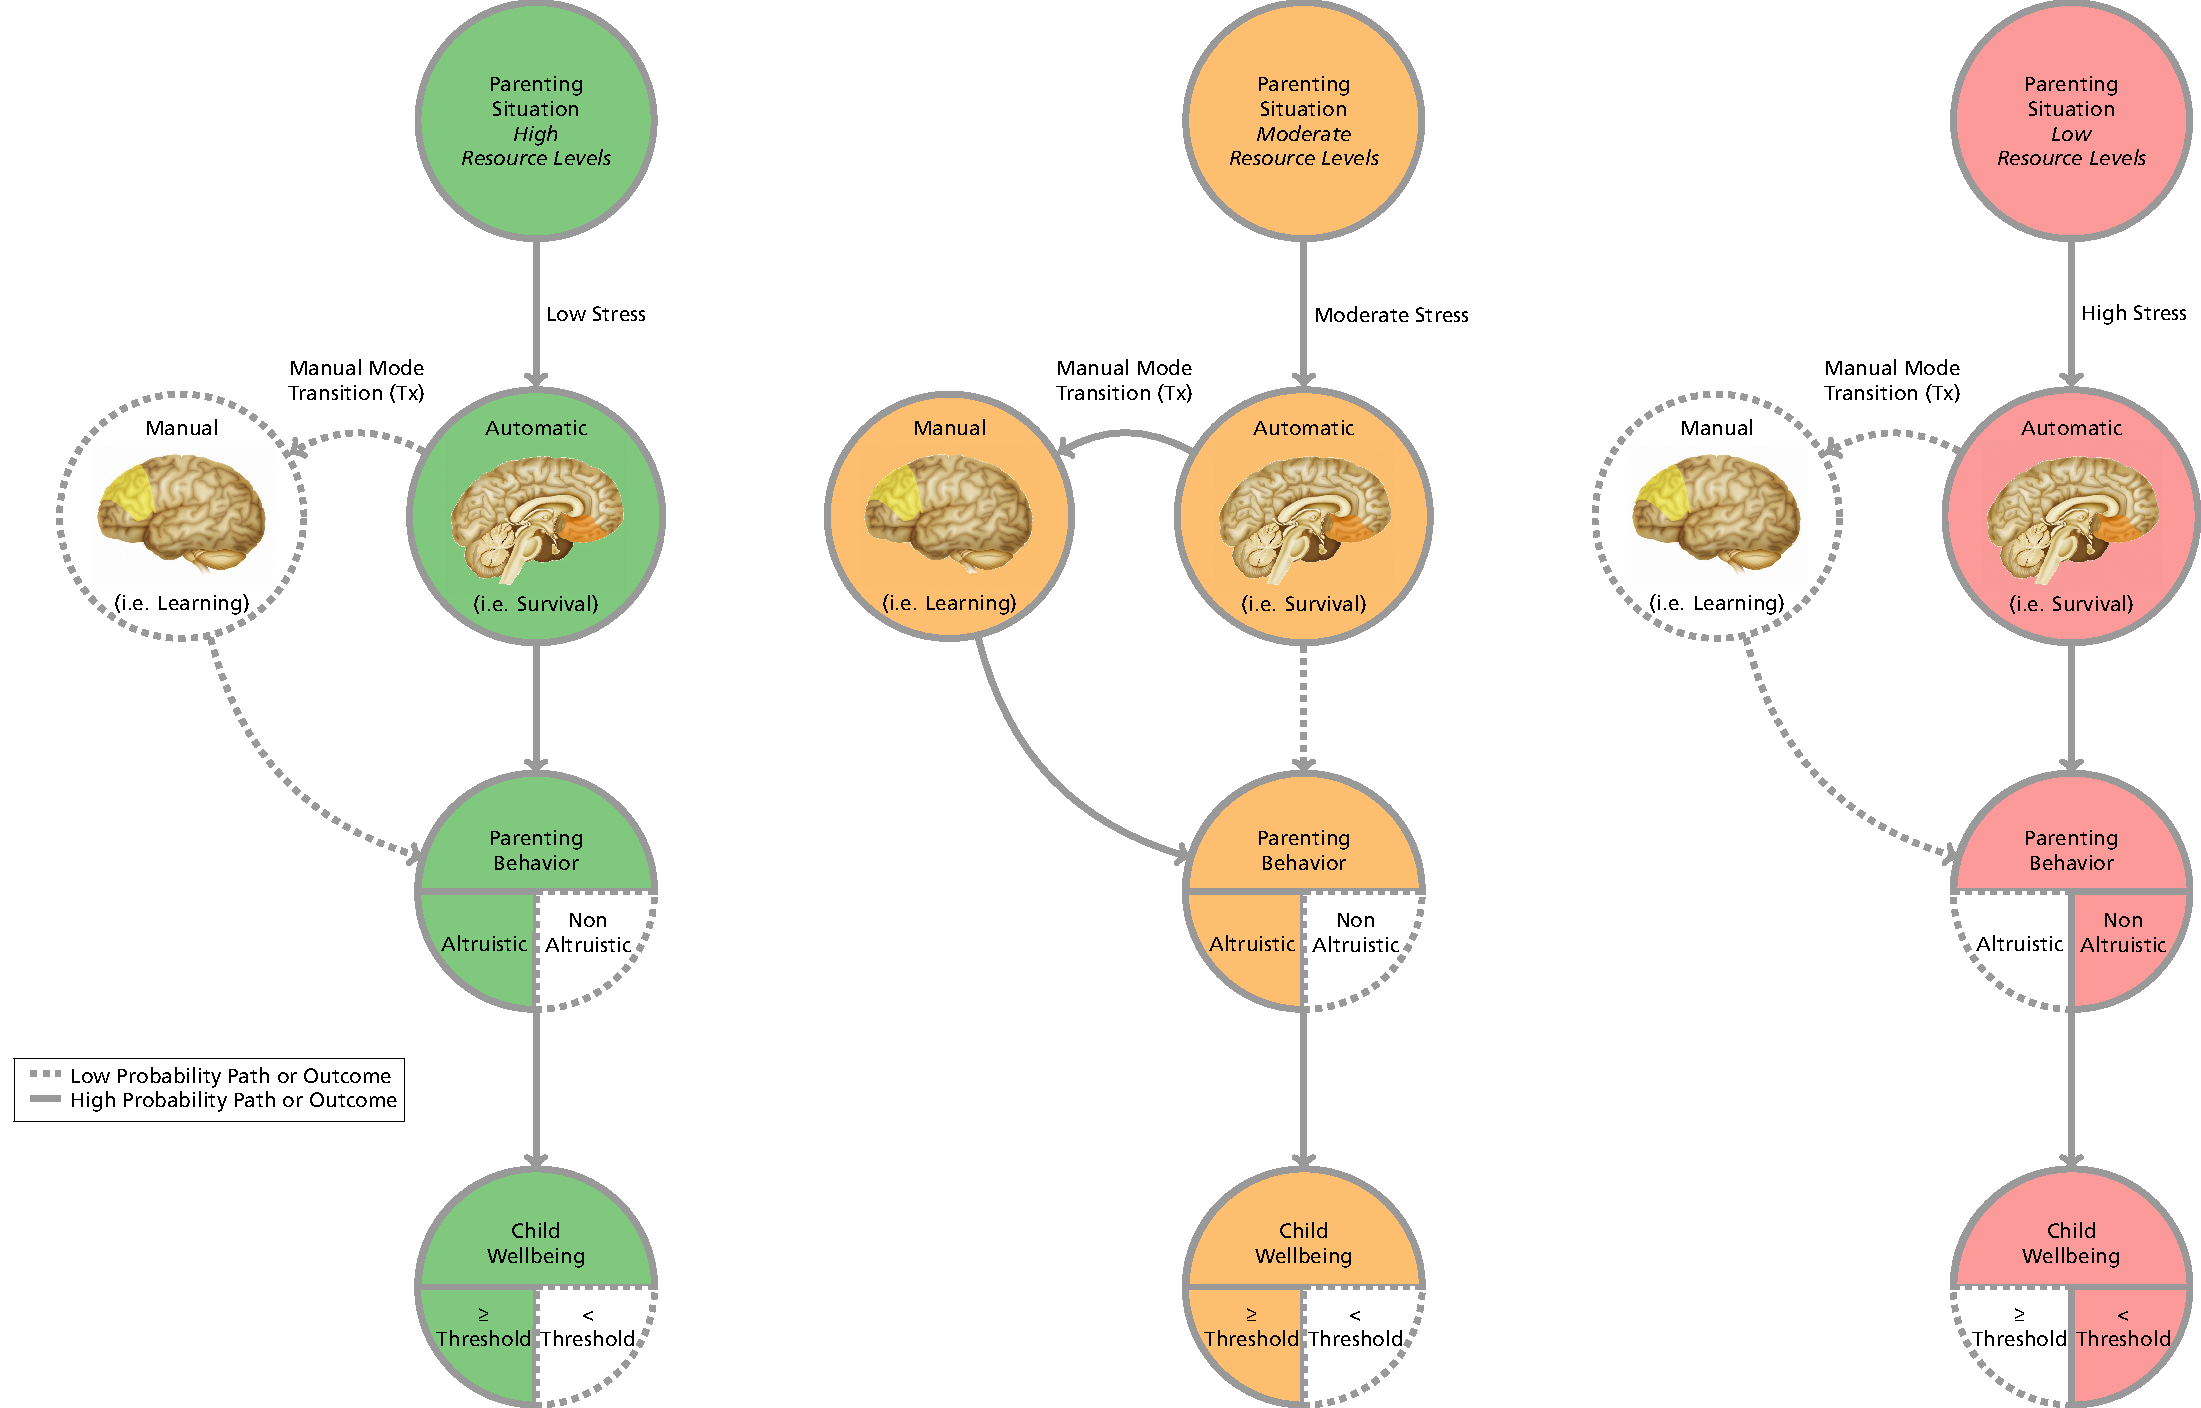
\includegraphics[scale=0.45]{general_conceptual_model_flow.pdf}}
\caption{Conceptual diagram showing the manner in which parental decision making varies as a function of resources.}
\label{fig:fig1}
\end{figure}  
%\end{landscape}
\FloatBarrier
While the logic of the current manuscript assumes the existence of an
underlying theoretical structure similar to that in Figures \ref{fig:fig1} and \ref{fig:fig2},
only two components of the above theoretical model will be specifically
tested: parenting situation (i.e.~resource level) and parenting
behavior. Specifically, this manuscript seeks to test the relationship
between parenting situation and parenting behaviors. The prediction of
the model above is that, as resource levels increase, altruistic
parenting behavior will also increase.
\FloatBarrier
\begin{figure}[htp] \centering{
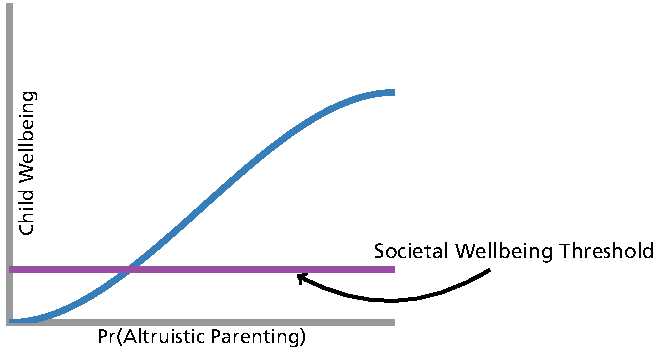
\includegraphics[scale=1.25]{general_conceptual_model_graph.pdf}}
\caption{Hypothetical graph of child wellbeing as a function of altruistic parenting.}
\label{fig:fig2}
\end{figure}  
\FloatBarrier
\section{Operational Definition of Key
Constructs}\label{operational-definition-of-key-constructs}

\subsection{Microeconomic Background}\label{microeconomic-background}

In order to test the relationship between parenting situation and
parental altruism, it is first necessary to develop an operational
definition of altruism for the purposes of this manuscript. This will be
accomplished by relying on basic household microeconomic theory. For
present purposes, an assumption is made that a particular household
contains two individuals: a parent and a child\footnote{This is a
  simplifying assumption made for the purposes of this manuscript. The
  model proposed here, however, readily extends to multiple children and
  multiple parents as well as to children of varying ages and genders.}.
A further assumption is made that the child and parent experience
increases in wellbeing as a function of their consumption of household
resources such as money, parenting time, etc. These resources could be
shared or consumed completely by either a parent or child (see (Gorman,
1976) for a description of how private and public goods could be
distributed throughout a household).

In using the term wellbeing, this manuscript draws an implicit
equivalence between the term and the traditional concept of utility
utilized in standard microeconomic theory. In this way, this manuscript
follows the line of literature started by Easterlin (1974) which
acknowledges that the choices that people make are subject to the
context in which an individual finds themselves and that an individual's
wellbeing is derived from more than just increased consumption. This
view implies that income-based measures of wellbeing should be thought
of as necessary but not sufficient to the study of wellbeing (Graham,
2008). In general, this manuscript proceeds from an assumption that
wellbeing can be conceptualized by what philosophers and positive
psychologists would refer to as eudaimonia - a higher level of happiness
(Kashdan, Biswas-Diener, \& King, 2008) which can be viewed as inclusive
of cognitive or hedonic forms of happiness. While this manuscript does
not explicitly test a eudaimonic formulation of wellbeing in economic
models, the reader should be clear that the models and theoretical
assumptions presented here are, in the general case, consistent with
notions of wellbeing and happiness that are more familiar to
non-economists and social welfare scholars (e.g. Ryff, 1989) and that
these conceptions of wellbeing do not necessarily reduce to hedonism or
require strictly ``rational'' preferences.

Like the economic conception of utility, wellbeing can be understood as
the level of satisfaction that an individual experiences as the result
of consumption and other choices about how to live their lives\footnote{It
  is important to note that human wellbeing is not just a function of
  the items that an individual might purchase or consume; it is more
  generally a function of an individual's preferences and the choices
  that individuals make throughout their lives. Talking in terms of
  consumption is simply a convenient way of discussing human choices and
  the constraints (e.g.~budgets, etc.) that people have on there
  choices.}. For present purposes, two composite goods that could be
consumed by a child are considered: household-produced investments
(e.g.~making meals, reading to the child, playing with the child, etc.)
and market purchased investments for the child (e.g.~childcare, etc.).
The logic of this manuscript implicitly follows Brandon (2001) and
assumes that a child's \emph{total} wellbeing is comprised of
household-produced investments and market purchased investments. This
does not imply that wellbeing is simply a function of financial
resources. This assumption simply implies that a child's \emph{total}
wellbeing is a function of all of the household resources (e.g.~time,
energy, money, etc.) that are directed to a child.

\subsection{Altruism}\label{altruism}

An important point from the discussion above is that parents can invest
in their child's wellbeing \emph{or} their own wellbeing. As noted
above, parental altruism can be defined as those behaviors requiring the
investment of time or other resources in a child in a way that benefits
the child but comes at a cost to the parent. Evolutionary theory defines
this benefit on the basis of the parent or child's fitness as a future
mate. Here, the notion of altruism is expanded to define this benefit in
terms of parent or child wellbeing. In other words, parental altruism is
defined as those parental behaviors or decisions requiring the
investment of time or other resources in a child in a way that increases
the wellbeing of the child but at a cost to parental wellbeing. This
expanded definition requires the implicit assumption that increases in
wellbeing will also tend to increase an individual's fitness as a future
mate. As described in more detail in the technical appendix, this
manuscript also proceeds from the assumption that parental altruism can
be operationally defined as the proportion of household resources
(including emotional resource, time, etc.) expended on a child. For the
purposes of this paper, resources expended on a child are assumed to be
completely consumed by the child. That is, the parent is not assumed to
benefit directly from the resource expenditure directed toward the
child. This is a simplifying assumption made to accommodate the data
utilized in this study. The theory presented here is, however, general
enough to accommodate resource expenditures which benefited the parent
and the child in future analyses.

\subsection{Maltreative Behaviors}\label{maltreative-behaviors}

For the purposes of this manuscript, maltreative behaviors can be
defined as those behaviors that will ultimately bring a child's
cumulative well-being below the societally defined threshold discussed
above. The current manuscript will focus specifically on parental
discipline strategies. Following the field of behavioral psychology,
this manuscript distinguishes parental discipline strategies into those
strategies involving the provision of a stimulus (e.g.~spanking,
yelling, etc.) and those involving the removal of a stimulus
(e.g.~time-out, removing a toy, etc.). The behaviorist literature
classifies these strategies as Type I and Type II discipline
respectively. Generally speaking, Type I strategies are less-likely to
promote child well-being than Type II discipline strategies. For
example, Type I strategies tend to be problematic for parent-child
relationships and can sometimes lead to behavioral problems for children
including delinquency and aggression (Gershoff, 2002; Taylor,
Manganello, Lee, \& Rice, 2010) - phenomena which are assumed to be
negatively associated with a child's cumulative wellbeing.

\subsection{Connecting Altruism to Maltreative Parental
Behaviors}\label{connecting-altruism-to-maltreative-parental-behaviors}

Following Brandon (2001) and Brandon (1999) and the discussion above, an
assumption is made here that a given society sets a minimum wellbeing
threshold. When parents invest in their children above this level,
society is generally accepting of the parent. When parents invest below
this level, the state must intervene to ensure a minimum level of
wellbeing for the child. Figure \ref{fig:fig4} illustrates this point in terms of a
wellbeing production possibility possibility. Each curve (Possibility 1
and Possibility 2) represent the possible outcomes of parental and child
wellbeing that could be produced within a lower (Possibility 1) and
higher (Possibility 2) level of resources. 

\begin{figure}[htp] \centering{
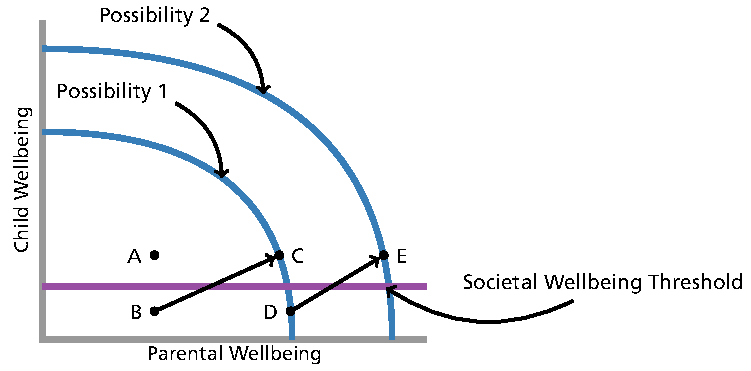
\includegraphics[scale=1.25]{wellbeing_production_possibilities.pdf}}
\caption{Parental and child possible wellbeing outcomes (i.e. production possibilities).}
\label{fig:fig4}
\end{figure}  

Several points are immediately clear from this diagram. To begin, it can
be seen that households operating below a given curve may not be using
all available household resources. Such behavior, however, does not
necessarily constitute maltreatment. This is the case of point $A$ which
represents a hypothetical household which is not maximizing the
potential wellbeing for the parent or for the child. However, the
household is still producing above the minimal societal expectations. An
example of such a household may be a mother who recreationally uses
alcohol and marijuana in such a way that she fails to raise the
wellbeing of her self or her child to the maximum level allowable under
a given level of resources but is still able to make parenting decisions
which keep her child above society's minimal expectations. Sometimes,
however, failing to use all available resources does cause a household
to fall below societal expectations for child wellbeing. An example
might be a more extreme form of illegal drug use such as the regular
consumption of illicit methamphetamine hydrochloride (i.e. ``crystal
meth'') to the point where a child's basic needs are not being met.
Point $B$ could represent such a situation. By moving to point $C$, $B$
could be brought above societal expectations within the existing
resources of the household. In other words, they could stop maltreating
their child without any financial assistance. Such movement might take
place, for example, as the result of a drug treatment program in which a
substance-abusing parent achieves sobriety and is able to spend more
time with their child. Point $D$ represents a point where the parent is
using all of her available resources by investing along Possibility 1
but is still investing below societal expectations. In such an instance,
the state could provide a wealth transfer to the parent and, holding
parental altruism constant, increase the investment in the child above
societal expectations (to point $E$). The state could also seek to move
the parent from $D$ to $C$ by trying to change household and/or parental
preferences. An example of this might be the application of a parenting
intervention to teach the parent new discipline strategies.

Most importantly for the current manuscript, is the notion that a given
household will invest more or less in a child depending on a parent's
level of altruism (this will also depend on a household sharing rule as
discussed in the technical appendix). This point is well articulated by
consideration of points $C$ and $D$ in Figure \ref{fig:fig4}. These individuals
represent different combinations of parental and child wellbeing in
households with exact same level of resources. According to the
assumptions outlined above, the difference between these two points
takes place as the result of differences in altruism between the parents
represented by $C$ and $D$ - Parent $C$ has a greater level of altruism
than $D$. As drawn in this figure, $D$ has such a low level of altruism
that they invest in their child below the societal threshold\footnote{In
  addition to altruism, Brandon (2001) developed the concept of parental
  efficiency in various childcaring strategies. The concept of parental
  efficiency was tested in analysis related to this manuscript and is
  described in the technical appendix to this manuscript. Efficiency, as
  defined in these analyses, proved to have no significant predictive
  power with respect to parental discipline strategies. While parental
  efficiency may have bearing on future analyses, substantive
  discussions of efficiency are excluded from this manuscript for the
  sake of brevity.}. A single investment below the threshold may or may
not constitute child maltreatment. However, every investment is assumed
to contribute either positively or negatively to a child's cumulative
wellbeing.

As described in the previous section, the parental investment of
interest for the current manuscript is parental discipline strategy.
This manuscript proceeds from the assumption that, while Type II
discipline strategies are more likely to maximize a child's wellbeing,
they are also more resource intensive than Type I discipline strategies
and more likely to require manual mode thinking (i.e.~higher-level
thinking). For example, spanking a child can be reasonably thought of as
a discipline strategy which stems from automatic mode thinking and
requires a relatively low level of cognitive resources. A ``time-out'',
however, can be reasonably thought of as a strategy requiring at least
some manual mode thinking and, as compared to spanking, a high level of
cognitive resources (e.g.~monitoring the child in their state of time
out, etc.). In other words, Type II discipline strategies can be
reasonably thought of as more altruistic than Type I parenting
strategies. As stated, the main hypothesis of this manuscript is that,
as resource levels increase, altruistic parenting behavior will also
increase. While prior research has reliably identified a link between
Type I strategies and low levels of resources (Berger, 2007; Berger, Paxson, \& Waldfogel, 2009; Berger, Brooks-Gunn, Paxson, \&
Waldfogel, 2008; Paxson \& Waldfogel, 2002), in the current analysis, an
independent effect of altruism while controlling for the effects of
resources is expected.

\section{Methods}\label{methods}

\subsection{Data and Analytical
Strategy}\label{data-and-analytical-strategy}

The National Survey of Early Childhood Health (NSECH) serves as the main
data for this analysis. This survey involved telephone interviews with
over 2,000 parents with children under 3 years of age in early 2000
(n=2,068). In addition to various demographic factors, the NSECH also
collected information on the income of parents and their employment
status, the time that children spend in the care of other individuals,
the source of the care (childcare provider, etc.), the time that parents
spend caring for their children in various activities (story-reading,
etc.), and parental discipline strategies, (spanking, time-out, etc.).

A main barrier with the NSECH data is that the survey provides
information on income, childcare, time-investments, and discipline
strategies in ordinal scales which limits the possibility of basic
mathematical operations requisite for the analysis conducted here
(e.g.~summing). The ordinal nature of the NSECH data is addressed by
making use of other nationally representative data sets. Specifically,
Bureau of Labor Statistics (BLS) data from the 2003 American Time Use
Survey (ATUS) and the 2004 Consumer Expenditure Survey (CE) is utilized.
Using this data to develop ``prior'' distributions for each measure, the
following smoothing algorithm is implemented which provides a method to
treat the data from these surveys as continuous:

\begin{enumerate}
\def\labelenumi{\arabic{enumi}.}
\itemsep1pt\parskip0pt\parsep0pt
\item
  Match the relevant variables from the NSECH and the relevant BLS
  survey,
\item
  Visually examine the distribution of the BLS data,
\item
  Calculate the MLE of a reasonable prior for the relevant variable,
\item
  Simulate a sampling distribution of relevant variable with a Monte
  Carlo function, and
\item
  Sample from the simulated data sets within intervals as identified in
  the ordinal NSECH data.
\end{enumerate}

Two exceptions are made to this algorithm. The first exception is in the
estimate of the total household expenditures on child care. For this
measurement, CE-based estimates of the average expenditures for
childcare in various childcare settings were obtained and multiplied by
the total hours that NSECH respondents reported that their child spent
in the corresponding settings. The variance in the hours reported in
NSECH provides a continuous measurement of this expenditure without the
need to incorporate the variance of a CE-based ``prior''. Also, in
estimating a continuous measurement of income, a distribution as
reported in a working paper by Bandourian, McDonald, \& Turley (2002) is
utilized which provides a reasonable prior distribution for US income.

Further details of the data preparation strategy (and subsequent steps
in the analysis) are available in a
\href{https://github.com/mienkoja/qualpaper}{GitHub repository} and will
also be included in the technical appendix to this manuscript.

\subsection{Descriptions of Key
Variables}\label{descriptions-of-key-variables}

\subsubsection{Household Income}\label{household-income}

Income in the public-use NSECH data is reported in terms of total
household income on an 8-point Likert scale starting at $\le$ 7,500 and
proceeding in increments of 10,000 to $\ge$ 75,000. Continuous income is
calculated using the algorithm specified above. As income is reported as
``total household income'', depending on the use, the estimated
continuous value is divided by the number of adults in the household in
order to arrive at an estimate of individual wages for parents who
report some employment.

\subsubsection{Altruism (i.e.~Household Resources Devoted to Child
Well-Being)}\label{altruism-i.e.household-resources-devoted-to-child-well-being}

Given the assumptions described above and in the technical appendix, the
total household resources devoted to the child can be thought of as a
measurement of ``household altruism'' toward the child. In order to
calculate altruism, the following steps are followed:

\begin{enumerate}
\def\labelenumi{\arabic{enumi}.}
\item
  Taking the estimate of household income calculated above, the count of
  adults in the home, and the estimated number of work hours, parent's
  wage is estimated as $(\text{income}/\text{count of adults})$ divided
  by $(365.25\cdot(\text{work hours}))$. For non-working mothers, time
  is valued based on the estimated market rate for childcare calculated
  from the CE.
\item
  Altruism is then calculated by summing child care expenditures
  $(\text{home based child care} + \text{market child care})$ and then
  dividing that value by the value of hours in a year
  $(\text{parental wage from step 1})\cdot(365.25)\cdot(24)$.
\end{enumerate}

\subsubsection{Probability of All Type II
Discipline}\label{probability-of-all-type-ii-discipline}

In order to obtain a single indicator of a parent's propensity to engage
in Type II discipline strategies, survey information concerning the
discipline strategies of the parent is used. Specifically, for each
person, the probability that \emph{all} of their reported discipline
strategies would be Type II is calculated.

Parents in the NSECH were asked 5 questions regarding their discipline
strategies. The specific question pattern is as follows:

\begin{quote}
The next questions are about discipline. Parents vary a lot in how they
discipline and children also vary in their response to being
disciplined. I am going to read a list of methods of discipline parents
might use with children (CHILD)'s age. For each, please tell me if you
use that method often, sometimes, rarely, or never with (CHILD). First,
how about raising your voice or yelling? How about spanking? How about
taking away a toy or treat? How about giving a time-out, that is making
(CHILD) take a break from whatever activity \{he/she\} is involved in?
How about explaining to (CHILD) why \{his/her\} behavior is not
appropriate.
\end{quote}

Using this information, the probability of all type II discipline is
calculated as follows:

\begin{enumerate}
\def\labelenumi{\arabic{enumi}.}
\itemsep1pt\parskip0pt\parsep0pt
\item
  In order from first to last, the first and second are classified as
  Type I strategies as they are are providing a stimulus to the child.
  The third and fourth questions are classified as Type II strategies as
  they remove a stimulus from the child\footnote{This paper categorizes
    behaviors into Type I and Type II strategies. From a strictly
    behavioral perspective, ``explaining'' strategies would be
    considered to be a form of positive discipline (i.e.~a Type I)
    strategy similar to yelling and spanking; the parent is giving
    instead of taking. Nonetheless, a salient argument could be made
    that forcing a child to engaging in verbal communication removes
    them from a stimulus and is thus a Type II strategy. Given the
    potential for confusion, the last question is removed from the
    analysis and focus is instead made on the four remaining behaviors
    which clearly fall within the Type I and Type II strategies. In
    cross-validation analyses, the results for models in which
    ``explaining'' is entered into the model as a Type I strategy, a
    Type II strategy, or excluded are nearly identical.}.
\item
  Each question response is then dichotomized. Questions in which a
  subject answered ``Never'' were coded as 0 and 1 otherwise.
\item
  The probability of all Type II discipline is calculated for each
  subject as the sum of dichotomized Type II responses, divided by the
  sum of dichotomized Type II responses plus the sum of dichotomized
  Type I responses
  $(\sum\text{Type II}/(\sum\text{Type II} + \sum\text{Type I}))$.
\end{enumerate}

\subsubsection{Additional Variables}\label{additional-variables}

In addition to the key variables of interest, additional variables
utilized in previous NSECH research concerning discipline strategies are
included in the analysis. Specifically, Regalado, Sareen, Inkelas,
Wissow, \& Halfon (2004) makes use of child age, maternal race, maternal
age, maternal marital status, maternal education, maternal frustration
levels, child health, and developmental concerns as potential risk
factors in their multivariate analysis. The current analysis also makes
use of the count of children in the household as an additional variable.
A descriptive summary of all the identified variables is provided in the
table below.

\begin{longtable}[c]{@{}lrrrr@{}}
\toprule\addlinespace
& Min & Max & Mean & Median
\\\addlinespace
\midrule\endhead
Probability of All Type II & 0.00 & 1.00 & 0.47 & 0.50
\\\addlinespace
Altruism & 0.02 & 1.00 & 0.28 & 0.25
\\\addlinespace
Efficiency\footnote{Ibid.} & 0.17 & 0.92 & 0.67 & 0.70
\\\addlinespace
Income & 132.11 & 186747.69 & 36412.74 & 26111.33
\\\addlinespace
Child Count & 1.00 & 4.00 & 2.18 & 2.00
\\\addlinespace
Child Age (mos) & 19.00 & 35.00 & 26.62 & 27.00
\\\addlinespace
White Mother & 0.00 & 1.00 & 0.54 & 1.00
\\\addlinespace
Maternal Age & 17.00 & 49.00 & 29.26 & 29.00
\\\addlinespace
Married Mother & 0.00 & 1.00 & 0.63 & 1.00
\\\addlinespace
Maternal College & 0.00 & 1.00 & 0.48 & 0.00
\\\addlinespace
Maternal Frustration & 0.00 & 1.00 & 0.54 & 1.00
\\\addlinespace
Child Healthy & 0.00 & 1.00 & 0.81 & 1.00
\\\addlinespace
Devolpmental Concerns & 0.00 & 1.00 & 0.79 & 1.00
\\\addlinespace
\bottomrule
\end{longtable}

\subsection{Statistical Analysis}\label{statistical-analysis}

All of the identified covariates were subjected to Bayesian Model
Averaging (BMA) across generalized linear models (GLMs) to determine the
most probable set of covariates. The details of BMA are beyond the scope
of this manuscript. The reader is directed, however, to J. A. Hoeting,
Madigan, Raftery, \& Volinsky (1999) for a discussion of the overall
approach. Briefly, BMA is a process through which a researcher
identifies a set of potential $k$ covariates and a candidate statistical
model (e.g.~a quasibinomial generalized linear model (GLM)). The analyst
then estimates the statistical model for every possible combination of
models ($2^k$ models). Each model receives a weighting based on the
posterior probability of the model beginning with a prior probability
which represents the researcher's beliefs prior to conducting the
analysis. For the current problem, the analysis utilizes a relatively
conservative uniform prior. A quasibinomial GLM is chosen for the BMA to
account for overdispersion in the Probability of all Type II Discipline.
The BMA is implemented via the R \texttt{BMA} package authored by A.
Raftery, Hoeting, Volinsky, Painter, \& Yeung (2009).

\section{Results}\label{results}

The results of the BMA indicate that the ``most probable'' of the $2^k$
fitted models is a model which only includes Altruism and Income.
Specifically, this model has a posterior probability of 0.472 and the
next most-probable model has a posterior probability of 0.16. The
estimates for the chosen model are displayed in the table below. All
parameters are statistically significant at the 0.0001 level. As can be
seen, the probability of choosing all Type II strategies positively and
significantly associated with altruism and income. The results are
displayed graphically in the figures below.

\begin{longtable}[c]{@{}lrrr@{}}
\toprule\addlinespace
& Estimate & Std. Error & t value
\\\addlinespace
\midrule\endhead
Intercept & -1.3877 & 0.2091 & -6.6379
\\\addlinespace
Altruism & 0.4446 & 0.1073 & 4.1450
\\\addlinespace
Income & 0.0803 & 0.0194 & 4.1328
\\\addlinespace
\bottomrule
\end{longtable}

\begin{figure}[htp] \centering{
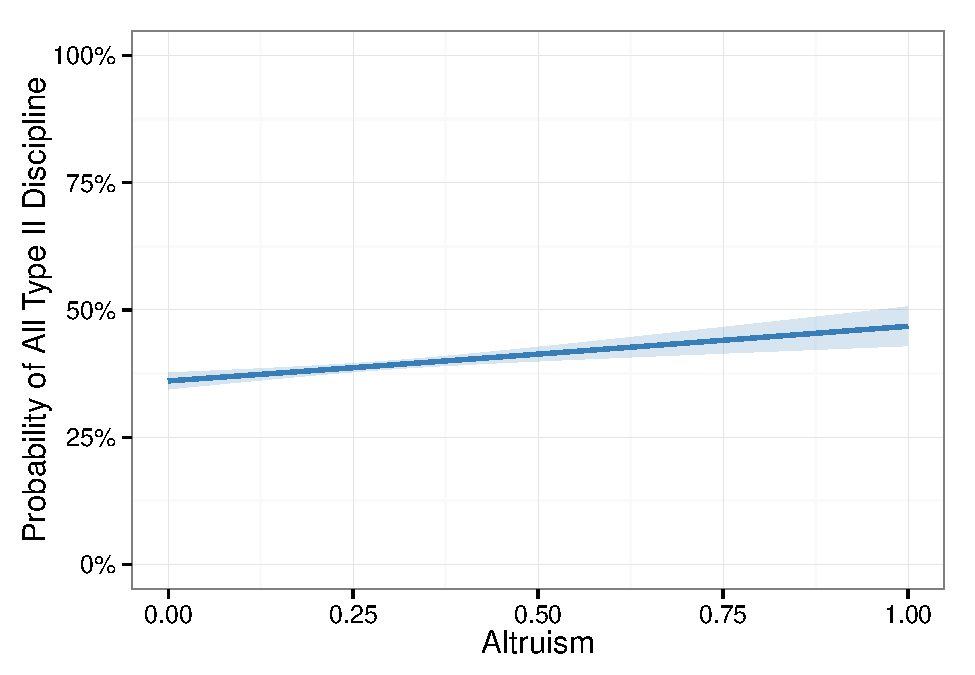
\includegraphics[scale=.75]{./qualpaper_v5_files/figure-latex/ModelResultGph2.pdf}
\caption{Predicted probabilities from final model.}
\label{fig:fig8}
\end{figure}  

\section{Discussion}\label{discussion}

The results of the analysis presented above confirm the hypothesis that
more altruistic households will tend to engage in parenting strategies
associated with wellbeing to a greater extent than less altruistic
households. This effect of altruism observed above is independent of the
income effect observed by other researchers. To the extent that the
other assumptions of the theoretical model hold, the results of this
analysis suggest that relatively simple models of human behavior might
be able to explain how families become involved with the child welfare
system.

What should be clear to the reader at this point is that the model
developed and tested in this manuscript is implicitly defining child
maltreatment as a problem of poverty. While previous researchers have
certainly drawn the connection between child welfare and poverty, such
literature usually attempts to examine the link between poverty and
deviant parental behaviors. Here, an alternative approach is taken in
defining maltreatment based on the manner in which poverty effects a
given child (in terms of their well-being) and the biological and social
context from which the parental behaviors emanate (resource constraints
and level of parental altruism).

In defining maltreatment in this manner, this manuscript breaks from
established lines of thinking about child maltreatment. Indeed, many
statutes specifically preclude poverty and homelessness as factors to be
considered when making legal determinations as to whether or not a given
child has been maltreated. While it is understandable that policy makers
would not want to hold a parent accountable for factors outside of their
control, focusing exclusively on parental behaviors ignores the
experience of a child in a given household and the causes of these
behaviors. The model presented here also elucidates the dynamic nature
of households and the variety of potential intervention points available
to the child welfare social work community.

\section{Limitations and Future
Directions}\label{limitations-and-future-directions}

Despite the usefulness of the model, it does suffer from an implicit
assumption of a parent who desires to invest (at least some) resources
in their child. The model presented here would suggest that all parents
would have a propensity to harm their children under a certain mix of
altruism and resource constraints, but that they typically seek to make
investments in children which maximize the child's wellbeing. However,
some parents suffer from various forms of psychopathology which may
yield a desire to harm children under any circumstances. Instances of
pedophilic sadism seem to be evidence that such individuals do exist.
For those individuals, a model of maltreatment focused on the Kempe,
Silverman, Steele, \& Droegmuellar (1962) ``defect of character'' seems
more appropriate than the one presented here. The point of this
manuscript, however, is that there is no reason to believe that such
individuals are a normal part of society or even a normal part of the
Western child welfare system. Such individuals likely represent the
margins of both populations and policies and interventions should be
developed with this theoretical framework in mind.

The analysis presented here is consistent with a resource constraint
theory of child maltreatment. However, the available data did not allow
for a direct test of all aspects of the model. A direct test of the
model would require information on how much parents prefer one form of
discipline to another given the relative monetary or cognitive ``costs''
or ``benefits'' of a given strategy and how these preferences vary as a
function of resource constraints. Specifically, future research could
explore the line of experiments conducted by Greene (2014). One
could, for example, imagine a brain-imaging experiment in which
parent-subjects were placed under cognitive load and asked to make
decisions about various parenting strategies. Understanding how
parenting decisions are made within the dual-process theory of morality
(or a similar framework) seems critical to the understanding of
maltreatment. Additional research could be undertaken to properly
monetize various parenting strategies and specifically test the
assumption that more resource intensive parenting strategies tend to
increase the wellbeing of children.

From a practice perspective, the results of this analysis suggest that
some families may be helped more by increases in income or other
concrete resources than the sorts of psychotherapeutic interventions
which tend to be prevalent in child welfare service plans. The study
does not refute the value of psychotherapeutic interventions. It does,
however, suggest that other forms of intervention may work better in
certain families. Although the BMA does exclude maternal frustration as
a covariate in the final selected model, the analysis does not imply
that such factors (including forms of psychopathology) could play a
causal role in a parent's level of altruism. For those parents where
income is not a concern, this model would suggest that interventions
should focus on changing preferences (i.e.~altruism or caring and
sharing) of parents and households.

The results of the BMA presented here also deserve more detailed
examination. Although the BMA suggests a final model which excludes many
of the control variables which would typically be included in a
statistical model of parenting behavior (e.g.~age, race, gender, etc.),
the BMA does not rule out the possibility that such demographic
variables may play a causal role in altruism per se. Such a question
could be further explored through a multiple equation model (e.g.~path
analysis, etc.). Finally, additional research is needed (through the
direct study of social workers or other means) to understand the
societal variability of the wellbeing threshold. In other words, since
the model presented here proceeds from the assumption that the wellbeing
threshold is societally defined, research should be conducted to help
the field understand precisely how the threshold varies within and
between countries throughout the world; both presently and across time.

\section{Technical Appendix}\label{technical-appendix}

The following appendix is a slightly more technical version of certain
portions of the ``Operational Definition of Key Constructs'' and ``Data
and Analytical Strategy'' sections in the main body of the manuscript.
As the manuscript proper has been written to appeal to a wide audience,
the use of symbolic notation has been limited except where absolutely
necessary. The use of symbolic notation is expanded in this section to
provide some more specificity while still remaining within the
understanding level of the expected readership of this document.

\subsection{Microeconomic Background}\label{microeconomic-background-1}

This manuscript considers two types of individuals ($i$): $p$ and $c$
indicating a parent and child respectively. This is a simplifying
assumption made for the purposes of this paper. The model proposed here,
however, readily extends to multiple children and multiple parents as
well as to children of varying ages and genders. The parent's total
well-being is given as $w_p(x_p)$ where $x_p$ is a composite good
consumed by the parent. The child's well-being is given as $w_c(x_c)$
where $x_c$ is a composite good consumed by the child. For the purposes
of this paper, it is assumed that $x_p$ and $x_c$ are private goods. In
other words, $x_p$ is only consumed by $p$ and $x_c$ is only consumed by
$c$. The overall framework utilized here is, however, general enough to
accommodate both private and public goods through the application of a
Gorman (1976) type linear technology function.

In using the term wellbeing, this manuscript draws an implicit
equivalence between the term and the traditional concept of utility
utilized in standard microeconomic theory\footnote{In economic terms,
  this manuscript assumes that wellbeing (as measured by characteristics
  which are observable in practice or in principle) is a positive
  monotonic transformation of an underlying latent utility concept
  $u_i$. Following the notation of the technical appendix, a further
  assumption is made that a person's wellbeing for two choices $j$ and
  $k$ is ordinally comparable such that
  $w_{ij} > w_{ik} \rightarrow u_{ij} > u_{ik}$, and that it is
  cardinally comparable with
  $w_{ij} - w_{ik} \rightarrow u_{ij} - u_{ik}$.}. In this way, this
manuscript follows the line of literature started by Easterlin (1974)
which acknowledges that the choices that people make are subject to the
context in which an individual finds themselves and that an individual's
wellbeing is derived from more than just increased consumption. This
view implies that income-based measures of wellbeing should be thought
of as necessary but not sufficient to the study of wellbeing (Graham,
2008). In general, this manuscript proceeds from an assumption that
wellbeing can be conceptualized by what philosophers and positive
psychologists would refer to as eudaimonia - a higher level of happiness
(Kashdan et al., 2008) which can be viewed as inclusive of cognitive or
hedonic forms of happiness. While this manuscript does not explicitly
test a eudaimonic formulation of wellbeing in economic models, the
reader should be clear that the models and theoretical assumptions
presented here are, in the general case, consistent with notions of
wellbeing and happiness that are more familiar to non-economists and
social welfare scholars (e.g. Ryff, 1989) and that these conceptions of
wellbeing do not necessarily reduce to hedonism or require strictly
``rational'' preferences.

Like the economic conception of utility, well-being can be understood as
the level of satisfaction that an individual experiences as the result
of consumption and other choices about how to live their lives. For
present purposes, two composite goods that could be consumed by a child
are considered: household-produced investments $x_{ch}$ (e.g.~making
meals, reading to the child, playing with the child, etc.) and market
purchased investments for the child $x_{cm}$ (e.g.~childcare, etc.).
This paper implicitly follows Brandon (2001) and assumes that
$x_c = x_{ch} + x_{cm}$ such that $w_c=w(x_{ch},x_{cm})$.

For illustrative purposes\footnote{These figures are for illustrative
  purposes only. Except where specifically noted, no functional form of
  the wellbeing functions proposed in this manuscript is assumed.}, the
contours of $w_c$ are shown in Figure \ref{fig:fig3}. As in utility theory, the
contours are referred to as indifference curves; a two-dimensional
representation of a three-dimensional well-being function. A key feature
of this graph is the notion of substitution. That is, as the child
consumes more of one form of investment, she necessarily consumes less
of the other. Movement along any one indifference curve represents a
household's trade-offs of one good for another while maintaining a
constant level of well-being. As the household investment in a child
moves from one curve to the next (i.e.~from $w1$, to $w2$, to $w3$), the
child's well-being is said to be increasing. The goods that comprise
$x_p$ can be assumed to behave in a similar manner.

\begin{figure}[htp] \centering{
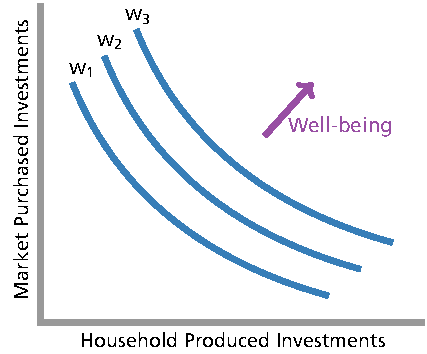
\includegraphics[scale=1.25]{basic_utility.pdf}}
\caption{Child wellbeing outcomes as a function of parental investment decisions.}
\label{fig:fig3}
\end{figure}  

This manuscript relies heavily on the collective model of the household
as first conceptualized by Chiappori (1988). In a collective
model, household members are assumed to cooperate in order to achieve a
Pareto efficient distribution of household resources. In this way this
manuscript breaks from Brandon (1999) and Brandon (2001) in which a
unitary model, in line with Becker (1981), is assumed to underlie
the household decision-making process. While a full review of unitary
and collective models of household decision-making is outside of the
scope of this paper (see Donni \& Chiappori (2011) for such a review),
unitary models have fallen out of favor in recent years. In general,
unitary models suffer from the assumption of a single decision-maker in
a given household. In developing a theory of child maltreatment, a
collective approach in which the preferences of the parent (or parents)
\emph{and} the preferences of the child (or children) are considered to
be analytically preferable to a unitary model in which child preferences
are typically ignored. Furthermore, with respect to maltreatment, the
basic conclusions of Brandon (1999) and Brandon (2001) still hold under
this model.

A specific assumption is made in this model that each member of the
household seeks to maximize the household welfare $W$ through a
two-stage program. In the first stage of the program, the household
identifies a sharing rule $\phi_i$ in which the parent's share of income
is governed by a sharing function $\phi_p=\phi(p_p, p_c, y, Z)$ and the
child's share of income is governed by a sharing function
$\phi_c=y-\phi(p_p, p_c, y, Z)$ where $p_p$ and $p_c$ represent
labor-based wages of the parent and child respectively, $y$ represents
household income, and $Z$ represents a vector of distribution factors
which do not impact parental or child preferences but do influence the
manner in which resources are distributed within the household. Such
factors could include local child protection laws, the age of the child,
cultural factors, and other considerations. The second stage of the
program involves each member maximizing a household welfare function
$W^i$ according to the following program:

\begin{align}\label{eqn:stage2}
\begin{split}
\text{max } W^i[w_p(x_p), w_c(x_c)]\\
\text{s.t. } x_i = \phi_i
\end{split}
\end{align}

While some readers may question the implicit human agency afforded to
children in the above specification, this approach is preferred to
ignoring the preferences of children in the allocation of household
resources (as in, e.g. Blundell, Chiappori, Magnac, \& Meghir, 2007). As
shown by Sodian, Schoeppner, \& Metz (2004), even infants can be shown
to exhibit human agency. This point will be well-taken by any reader who
has ever parented a newborn child overnight; the preferences of the
child as manifest through a desire to feed, play, or engage in other
activities at any hour of the day or night clearly impact which
household resources are available for the parent and which are available
for the child.

What should be clear from the above discussion is that
$p_c=0 \rightarrow \phi_c=x_c/y$. In other words, when $p_c=0$, $\phi_c$
is simply the proportion of household resources expended on the child in
stage 1. Some additional resources (some portion of $\phi_p$) may be
expended on the child in stage 2 of the program according to a caring
parameter $\alpha_p$ (i.e.~altruism under Becker (1981)). Under an
assumption that $W$ takes a Cobb-Douglas form where $\alpha_p$ is
defined as the output elasticity of $w_c$, it can be shown through Roy's
identity (Roy, 1947) that $\alpha$ is simply the proportion of $\phi_p$
which is expended on $x_c$. Thus, for present purposes total household
expenditures on $x_c$ are assumed equal to $\alpha_p + \phi_c$.

Following Brandon (2001) and Brandon (1999), we assume that a given
society sets a minimum well-being threshold $\bar{w}$. When parents
invest in their children above this level, society is generally
accepting of the parent. When parents invest below this level, the state
must intervene to ensure a minimum well-being for the child.

\subsection{Major Predictions of the
Model}\label{major-predictions-of-the-model}

There are many predictions which stem from the model of child
maltreatment described above. For present purposes, the major prediction
of this model is that the probability $P$ of child maltreatment can be
expressed as

\begin{align}\label{eqn:prediction}
P(w_c < \bar{w})=g(\alpha_p, \phi_c, y, F(\phi_c + \alpha_p, x_c))
\end{align}

where $F$ is the Farrell output efficiency for a household (Farrell,
1957) in terms of the inputs $(\phi_c + \alpha_p)$ and output $x_c$. The
model presented here specifically predicts that $P(w_c < \bar{w})$
monotonically decreases as a function of $g$.

\subsection{Assumptions Regarding Discipline
Strategies}\label{assumptions-regarding-discipline-strategies}

This analysis proceeds from the assumption that discipline strategies
can be classified according to the provision of a stimulus
(e.g.~spanking, yelling, etc.) as compared with the taking of a stimulus
(e.g.~time-out, removing a toy, etc.). The behaviorist literature
classifies these strategies as Type I ($D_I$) and Type II ($D_{II}$)
discipline respectively. This analysis assumes further that $D_I$
strategies are generally less-likely to promote child well-being than
$D_{II}$ discipline strategies. It is known, for instance, that $D_I$
strategies tend to be problematic for parent-child relationships and can
sometimes lead to behavioral problems for children including delinquency
and aggression (Gershoff, 2002; Taylor et al., 2010). This manuscript
thus proceeds from an assumption that $D_I$ and $D_{II}$ discipline
strategies exist on a spectrum of parenting behaviors and that $D_I$
behaviors are the sorts of behaviors that are less likely to increase a
child's well-being and more likely to create a situation in which
$w_c < \bar{w}$. This assumption is bolstered by a line of literature
which links $D_I$ parenting strategies to resource constraints (Berger, 2007; Berger et al., 2009; Berger et al., 2008; Paxson
\& Waldfogel, 2002) in a manner similar to the identified link between
resource constraints and child maltreatment in the literature reviewed
above.

\subsection{Description of Key
Variables}\label{description-of-key-variables}

The variables listed in the ``Major Predictions of the Model'' section
above are defined as follows:

\subsubsection{Household Income $(y)$}\label{household-income-y}

Income in the public-use NSECH data is reported in terms of total
household income on an 8-point Likert scale starting at $\le 7,500$ and
proceeding in increments of 10,000 to $\ge 75,000$. Continuous income is
calculated to the algorithm specified above. As income is reported as
``total household income'', depending on the use, the estimated
continuous value is divided by the number of adults in the household in
order to arrive at an estimate of individual wages for parents who
report some employment.

\subsubsection{Household Resources Devoted to Child Well-Being
$(\alpha_p + \phi_c)$}\label{household-resources-devoted-to-child-well-being-alphaux5fp-phiux5fc}

The values of $\alpha_p$ and $\phi_c$ are not observed directly in the
NSECH data. However, under the assumptions described above, it can be
said that the sum of these parameters is equal to the total household
resources devoted to the child $A$ (this can be thought of imprecisely
as a measure of ``household altruism'' toward the child). In order to
calculate $A$ the following steps are taken:

\begin{enumerate}
\def\labelenumi{\arabic{enumi}.}
\item
  Taking the estimate of $y$ calculated above, the count of adults in
  the home $n_a$, and the estimated number of work hours $t_w$, an
  estimate of the parent's wage $p_p$ is calculated as
  $(y/n_a)/(365.25(t_w))$. For non-working mothers, time is valued at
  the estimated market rate for child-care calculated from the CES
  above.
\item
  The value of $A$ is calculated by summing the total time value that a
  parent spends on home-based child care $p_px_{ch}$ and the time value
  of market child care $p_px_{cm}$ and then dividing by the time value
  of the total number of hours in the year $(p_p(365.25)(24))$ such that
  $A=(p_px_{ch}+p_px_{cm})/(p_p(365.25)(24))$.
\end{enumerate}

\subsubsection{Output Efficiency ($F$)}\label{output-efficiency-f}

The value of $F$ is not observed directly and there is no way to
empirically calculate this value within the available data. It is
possible, however, to estimate a distance function using an MLE of the
production possibility frontier for $x_{ch}$ and $x_{cm}$. While a
detailed discussion of this estimation is beyond the scope of this
paper, Bogetoft \& Otto (2010) provide a thorough overview of the
approach. In essence, several assumptions are made about the measure of
efficiency $F$. These assumptions (in conjunction with an estimate of
the frontier) are used to estimate a distance $D$ from the frontier for
each household in the data. This estimate is accomplished through the
use of the \texttt{Benchmarking} package by Bogetoft \& Otto (2013)
which is available in the statistical programming language, R.

\subsubsection{Probability of All Type II Strategies
$P(\text{All } D_{II})$}\label{probability-of-all-type-ii-strategies-ptextall-dux5fii}

Since there is no direct observations of societally identified
maltreatment, this paper utilizes information information concerning the
discipline strategies of the parent. For each person, the probability
that \emph{all} of reported discipline strategies would be $D_{II}$ is
calculated. In using this measurement as a dependent measure, there is
an implicit assumption that
$P(w_c \ge \bar{w}) \propto  P(\text{All } D_{II})$.

Parents in the NSECH were asked 5 questions regarding their discipline
strategies. The specific question pattern is as follows:

\begin{quote}
The next questions are about discipline. Parents vary a lot in how they
discipline and children also vary in their response to being
disciplined. I am going to read a list of methods of discipline parents
might use with children (CHILD)`s age. For each, please tell me if you
use that method often, sometimes, rarely, or never with (CHILD). First,
how about raising your voice or yelling? How about spanking? How about
taking away a toy or treat? How about giving a time-out, that is making
(CHILD) take a break from whatever activity \{he/she\} is involved in?
How about explaining to (CHILD) why \{his/her\} behavior is not
appropriate.''
\end{quote}

Using this information, $P(\text{All } D_{II})$ is calculated as
follows:

\begin{enumerate}
\def\labelenumi{\arabic{enumi}.}
\itemsep1pt\parskip0pt\parsep0pt
\item
  In order from first to last, the first, second, and last questions are
  classified as Type I strategies $D_I$ as they are are providing a
  stimulus to the child. The third and fourth questions are classified
  as Type II strategies $D_{II}$ as they remove a stimulus from the
  child.
\item
  Responses to each question were then dichotomized. Questions in which
  a subject answered ``Never'' were coded as 0 and 1 otherwise.
\item
  The probability for each subject $k$ is then calculated as\\
  $P_k(\text{All }D_{II_k})=\sum{D_{II_k}}/(\sum{D_{II_k}}+\sum{D_{I_k}})$.
\end{enumerate}

%\theendnotes

\section{References}\label{references}

Bandourian, R., McDonald, J. B., \& Turley, R. S. (2002). \emph{A
comparison of parametric models of income distribution across countries
and over time}. Maxwell School of Citizenship; Public Affairs, Syracuse
University.

Barro, R. J., Becker, G. S., \& Tomes, N. (1986). Human capital and the
rise and fall of families. \emph{Journal of Labor Economics},
\emph{4}(3).

Baumrind, D. (1993). The average expectable environment is not good
enough: A response to scarr. \emph{Child Development}, \emph{64}(5),
1299--1317.

Baumrind, D. (1995). \emph{Child maltreatment and optimal caregiving in
social contexts.} Garland Publishing.

Becker, G. S. (1981). \emph{A treatise on the family}. Harvard
university press.

Belsky, J., Steinberg, L., \& Draper, P. (1991). Childhood experience,
interpersonal development, and reproductive strategy: An evolutionary
theory of socialization. \emph{Child Development}, \emph{62}(4),
647--670.

Berger, L. M. (2007). Socioeconomic factors and substandard parenting.
\emph{Social Service Review}, \emph{81}(3), 485--522.

Berger, L. M., \& Waldfogel, J. (2004). Out-of-home placement of
children and economic factors: An empirical analysis. \emph{Review of
Economics of the Household}, \emph{2}(4), 387--411.

Berger, L. M., Paxson, C., \& Waldfogel, J. (2009). Income and child
development. \emph{Children and Youth Services Review}, \emph{31}(9),
978--989.

Berger, L., Brooks-Gunn, J., Paxson, C., \& Waldfogel, J. (2008).
First-year maternal employment and child outcomes: Differences across
racial and ethnic groups. \emph{Children and Youth Services Review},
\emph{30}(4), 365--387.

Blundell, R., Chiappori, P.-A., Magnac, T., \& Meghir, C. (2007).
Collective labour supply: Heterogeneity and non-participation. \emph{The
Review of Economic Studies}, \emph{74}(2), 417--445.

Bogetoft, P., \& Otto, L. (2010). \emph{Benchmarking with dEA, sFA, and
r} (Vol. 157). Springer.

Bogetoft, P., \& Otto, L. (2013). \emph{Benchmarking with dEA and sFA}.

Brandon, P. D. (1999). The state, the child, and imperfect parenting.
\emph{Rationality and Society}, \emph{11}(4), 399--418.

Brandon, P. D. (2001). State intervention in imperfect families: The
child, the state, and imperfect parenting reconsidered from a theory of
caomparative advantage. \emph{Rationality and Society}, \emph{13}(3),
285--303.

Burgess, R. L., \& Conger, R. D. (1978). Family interaction in abusive,
neglectful, and normal families. \emph{Child Development}, 1163--1173.

Cameron, G., \& Freymond, N. (2006). \emph{Towards positive systems of
child and family welfare: International comparisons of child protection,
family service, and community caring systems}. University of Toronto
Press.

Cancian, M., Yang, M.-Y., \& Slack, K. S. (2013). The effect of
additional child support income on the risk of child maltreatment.
\emph{Social Service Review}, \emph{87}(3), 417--437.

Chagnon, N. A. (1983). \emph{Yanomamö: The fierce people. new york:
Holt, rinehart and winston. 1991 yanomamö: The last days of eden}. San
Diego: Harcourt Brace.

Chiappori, P.-A. (1988). Rational household labor supply.
\emph{Econometrica: Journal of the Econometric Society}, 63--90.

Courtney, M. E., Dworsky, A., Piliavin, I., \& Zinn, A. (2005).
Involvement of tANF applicant families with child welfare services.
\emph{Social Service Review}, \emph{79}(1), 119--157.

Daly, M., \& Wilson, M. (1988). \emph{Homicide}. Transaction Publishers.

Donni, O., \& Chiappori, P.-A. (2011). Nonunitary models of household
behavior: A survey of the literature. In \emph{Household economic
behaviors} (pp. 1--40). Springer.

Easterlin, R. A. (1974). Does economic growth improve the human lot?
Some empirical evidence. \emph{Nations and Households in Economic
Growth}, \emph{89}.

Farrell, M. J. (1957). The measurement of productive efficiency.
\emph{Journal of the Royal Statistical Society. Series A (General)},
253--290.

Fein, D. J., \& Lee, W. S. (2003). The impacts of welfare reform on
child maltreatment in delaware. \emph{Children and Youth Services
Review}, \emph{25}(1), 83--111.

Ford, J. D., \& Courtois, C. A. (2009). \emph{Treating complex traumatic
stress disorders: An evidence-based guide}. Guilford New York.

Gershoff, E. T. (2002). Corporal punishment by parents and associated
child behaviors and experiences: a meta-analytic and theoretical review.
\emph{Psychological Bulletin}, \emph{128}(4), 539.

Gil, D. G. (1970). \emph{Violence against children: Physical child abuse
in the united states}. Harvard University Press Cambridge, MA.

Gorman, W. M. (1976). Tricks with utility functions. \emph{Essays in
Economic Analysis}, 211--243.

Graham, C. (2008). Happiness and health: Lessons---and questions---for
public policy. \emph{Health Affairs}, \emph{27}(1), 72--87.

Greene, J. D. (2014). Beyond point-and-shoot morality: Why cognitive
(neuro) science matters for ethics. \emph{Ethics}, \emph{124}(4),
695--726.

Hamilton, W. D. (1964). The genetical evolution of social behaviour. i.
\emph{Journal of Theoretical Biology}, \emph{7}(1), 1--16.

Ho, S. S., Konrath, S., Brown, S., \& Swain, J. E. (2014). Empathy and
stress related neural responses in maternal decision making.
\emph{Decision Neuroscience}, \emph{8}, 152.

Hoeting, J. A., Madigan, D., Raftery, A. E., \& Volinsky, C. T. (1999).
Bayesian model averaging: a tutorial. \emph{Statistical Science},
382--401.

Kashdan, T. B., Biswas-Diener, R., \& King, L. A. (2008). Reconsidering
happiness: The costs of distinguishing between hedonics and eudaimonia.
\emph{The Journal of Positive Psychology}, \emph{3}(4), 219--233.

Kempe, C., Silverman, F., Steele, B., \& Droegmuellar, W. (1962). The
battered child syndrome. \emph{The Journal of American Medical
Association}, \emph{181}, 4--11.

Mani, A., Mullainathan, S., Shafir, E., \& Zhao, J. (2013). Poverty
impedes cognitive function. \emph{science}, \emph{341}(6149), 976--980.

Milner, L. S. (1998). \emph{Hardness of heart/hardness of life: the
stain of human infanticide}. University Press of America.

Murdoch, L. (2006). \emph{Imagined orphans: Poor families, child
welfare, and contested citizenship in london}. Rutgers University Press.

Paxson, C., \& Waldfogel, J. (2002). Work, welfare, and child
maltreatment. \emph{Journal of Labor Economics}, \emph{20}(3), 435--474.

Paxton, J. M., Ungar, L., \& Greene, J. D. (2012). Reflection and
reasoning in moral judgment. \emph{Cognitive Science}, \emph{36}(1),
163--177.

Pelton, L. H. (1981). \emph{The social context of child abuse and
neglect}. Human Sciences Press New York.

Pelton, L. H. (1994). The role of material factors in child abuse and
neglect. \emph{Protecting Children from Abuse and Neglect: Foundations
for a New National Strategy}, 131--181.

Plomin, R., Owen, M. J., \& McGuffin, P. (1994). The genetic basis of
complex human behaviors. \emph{Science}, \emph{264}(5166), 1733--1739.

Raftery, A., Hoeting, J., Volinsky, C., Painter, I., \& Yeung, K. Y.
(2009). BMA: Bayesian model averaging. r package version 3.12.
\emph{URL: http://CRAN. R-Project. Org/Package= BMA}.

Regalado, M., Sareen, H., Inkelas, M., Wissow, L. S., \& Halfon, N.
(2004). Parents' discipline of young children: Results from the national
survey of early childhood health. \emph{Pediatrics},
\emph{113}(Supplement 5), 1952--1958.

Ridley, M. (2003). \emph{Nature via nurture: Genes, experience, and what
makes us human.} HarperCollins Publishers.

Roy, R. (1947). La distribution du revenu entre les divers biens.
\emph{Econometrica, Journal of the Econometric Society}, 205--225.

Russell, A. B., \& Trainor, C. M. (1984). \emph{Trends in child abuse
and neglect: A national perspective}. American Humane Association,
Children's Division.

Ryff, C. D. (1989). Happiness is everything, or is it? Explorations on
the meaning of psychological well-being. \emph{Journal of Personality
and Social Psychology}, \emph{57}(6), 1069.

Sedlak, A. J., \& Broadhurst, D. D. (1996). The national incidence study
of child abuse and neglect. \emph{Washington DC. US Department of Health
and Human Services}.

Sedlak, A. J., Mettenburg, J., Basena, M., Peta, I., McPherson, K.,
Greene, A., \& others. (2010). Fourth national incidence study of child
abuse and neglect (nIS-4). \emph{Washington, DC: US Department of Health
and Human Services. Retrieved on July}, \emph{9}, 2010.

Slack, K. S., Lee, B. J., \& Berger, L. M. (2007). Do welfare sanctions
increase child protection system involvement? A cautious answer.
\emph{Social Service Review}, \emph{81}(2), 207--228.

Sodian, B., Schoeppner, B., \& Metz, U. (2004). Do infants apply the
principle of rational action to human agents? \emph{Infant Behavior and
Development}, \emph{27}(1), 31--41.

Stith, S. M., Liu, T., Davies, L. C., Boykin, E. L., Alder, M. C.,
Harris, J. M., \ldots{} Dees, J. (2009). Risk factors in child
maltreatment: A meta-analytic review of the literature. \emph{Aggression
and Violent Behavior}, \emph{14}(1), 13--29.

Stuebe, A. M., Kleinman, K., Gillman, M. W., Rifas-Shiman, S. L.,
Gunderson, E. P., \& Rich-Edwards, J. (2010). Duration of lactation and
maternal metabolism at 3 years postpartum. \emph{Journal of Women's
Health}, \emph{19}(5), 941--950.

Suter, R. S., \& Hertwig, R. (2011). Time and moral judgment.
\emph{Cognition}, \emph{119}(3), 454--458.

Taylor, C. A., Manganello, J. A., Lee, S. J., \& Rice, J. C. (2010).
Mothers' spanking of 3-year-old children and subsequent risk of
children's aggressive behavior. \emph{Pediatrics}, \emph{125}(5),
e1057--e1065.

Testa, M., \& Poertner, J. (2010). \emph{Fostering accountability: Using
evidence to guide and improve child welfare policy}. Oxford Univ Pr.

Trivers, R. L. (1974). Parent-offspring conflict. \emph{American
Zoologist}, \emph{14}(1), 249--264.

Trocm{é}, N., Fallon, B., MacLaurin, B., Daciuk, J., Felstiner, C.,
Black, T., \ldots{} others. (2010). \emph{Canadian incidence study of
reported child abuse and neglect, 2008}. Public Health Agency of Canada
Ottawa.

Trocm{é}, N., Lajoie, J., Fallon, B., \& Felstiner, C. (2007). Injuries
and death of children at the hands of their parents.
\url{http://cwrp.ca/sites/default/files/publications/en/Injuries57E.pdf}.

US Department of Health and Human Services. (2013). \emph{Child welfare
outcomes 2008-2011-report to congress.} Author.


\end{document}
